%%%%%%%%%%%%%%%%%%%%%%%%%%%%%%%%%%%%%%%%%%%%%%%%%%%%%%%%%%%%%%%%%%%%%
%% This is a (brief) model paper using the achemso class
%% The document class accepts keyval options, which should include
%% the target journal and optionally the manuscript type. 
%%%%%%%%%%%%%%%%%%%%%%%%%%%%%%%%%%%%%%%%%%%%%%%%%%%%%%%%%%%%%%%%%%%%%
\documentclass[journal=langd5,manuscript=article]{achemso}

%%%%%%%%%%%%%%%%%%%%%%%%%%%%%%%%%%%%%%%%%%%%%%%%%%%%%%%%%%%%%%%%%%%%%
%% Place any additional packages needed here.  Only include packages
%% which are essential, to avoid problems later. Do NOT use any
%% packages which require e-TeX (for example etoolbox): the e-TeX
%% extensions are not currently available on the ACS conversion
%% servers.
%%%%%%%%%%%%%%%%%%%%%%%%%%%%%%%%%%%%%%%%%%%%%%%%%%%%%%%%%%%%%%%%%%%%%
\usepackage[version=3]{mhchem} % Formula subscripts using \ce{}
\usepackage{lineno}
\usepackage{booktabs}
\usepackage{hyperref}

%\linenumbers
%%%%%%%%%%%%%%%%%%%%%%%%%%%%%%%%%%%%%%%%%%%%%%%%%%%%%%%%%%%%%%%%%%%%%
%% If issues arise when submitting your manuscript, you may want to
%% un-comment the next line.  This provides information on the
%% version of every file you have used.
%%%%%%%%%%%%%%%%%%%%%%%%%%%%%%%%%%%%%%%%%%%%%%%%%%%%%%%%%%%%%%%%%%%%%
%%\listfiles

%%%%%%%%%%%%%%%%%%%%%%%%%%%%%%%%%%%%%%%%%%%%%%%%%%%%%%%%%%%%%%%%%%%%%
%% Place any additional macros here.  Please use \newcommand* where
%% possible, and avoid layout-changing macros (which are not used
%% when typesetting).
%%%%%%%%%%%%%%%%%%%%%%%%%%%%%%%%%%%%%%%%%%%%%%%%%%%%%%%%%%%%%%%%%%%%%
\newcommand*\mycommand[1]{\texttt{\emph{#1}}}
\renewcommand{\arraystretch}{1.2}

%%%%%%%%%%%%%%%%%%%%%%%%%%%%%%%%%%%%%%%%%%%%%%%%%%%%%%%%%%%%%%%%%%%%%
%% Meta-data block
%% ---------------
%% Each author should be given as a separate \author command.
%%
%% Corresponding authors should have an e-mail given after the author
%% name as an \email command. Phone and fax numbers can be given
%% using \phone and \fax, respectively; this information is optional.
%%
%% The affiliation of authors is given after the authors; each
%% \affiliation command applies to all preceding authors not already
%% assigned an affiliation.
%%
%% The affiliation takes an option argument for the short name.  This
%% will typically be something like "University of Somewhere".
%%
%% The \altaffiliation macro should be used for new address, etc.
%% On the other hand, \alsoaffiliation is used on a per author basis
%% when authors are associated with multiple institutions.
%%%%%%%%%%%%%%%%%%%%%%%%%%%%%%%%%%%%%%%%%%%%%%%%%%%%%%%%%%%%%%%%%%%%%


\author{Jack D. Evans}
\affiliation[TU Dresden]
{Department of Inorganic Chemistry,
Technische Universität Dresden,
Bergstraße 66, 01062 Dresden, Germany}
\email{jack.evans@tu-dresden.de}

\author{Volodymyr Bon}
\affiliation[TU Dresden]
{Department of Inorganic Chemistry,
Technische Universität Dresden,
Bergstraße 66, 01062 Dresden, Germany}

\author{Irena Senkovska}
\affiliation[TU Dresden]
{Department of Inorganic Chemistry,
Technische Universität Dresden,
Bergstraße 66, 01062 Dresden, Germany}

\author{Stefan Kaskel}
\affiliation[TU Dresden]
{Department of Inorganic Chemistry,
Technische Universität Dresden,
Bergstraße 66, 01062 Dresden, Germany}


%%%%%%%%%%%%%%%%%%%%%%%%%%%%%%%%%%%%%%%%%%%%%%%%%%%%%%%%%%%%%%%%%%%%%
%% The document title should be given as usual. Some journals require
%% a running title from the author: this should be supplied as an
%% optional argument to \title.
%%%%%%%%%%%%%%%%%%%%%%%%%%%%%%%%%%%%%%%%%%%%%%%%%%%%%%%%%%%%%%%%%%%%%
\title[]
  {A universal standard archive file for adsorption data}

%%%%%%%%%%%%%%%%%%%%%%%%%%%%%%%%%%%%%%%%%%%%%%%%%%%%%%%%%%%%%%%%%%%%%
%% Some journals require a list of abbreviations or keywords to be
%% supplied. These should be set up here, and will be printed after
%% the title and author information, if needed.
%%%%%%%%%%%%%%%%%%%%%%%%%%%%%%%%%%%%%%%%%%%%%%%%%%%%%%%%%%%%%%%%%%%%%
\abbreviations{IR,NMR,UV}
\keywords{American Chemical Society, \LaTeX}



%%%%%%%%%%%%%%%%%%%%%%%%%%%%%%%%%%%%%%%%%%%%%%%%%%%%%%%%%%%%%%%%%%%%%
%% The manuscript does not need to include \maketitle, which is
%% executed automatically.
%%%%%%%%%%%%%%%%%%%%%%%%%%%%%%%%%%%%%%%%%%%%%%%%%%%%%%%%%%%%%%%%%%%%%
\begin{document}

%%%%%%%%%%%%%%%%%%%%%%%%%%%%%%%%%%%%%%%%%%%%%%%%%%%%%%%%%%%%%%%%%%%%%
%% The "tocentry" environment can be used to create an entry for the
%% graphical table of contents. It is given here as some journals
%% require that it is printed as part of the abstract page. It will
%% be automatically moved as appropriate.
%%%%%%%%%%%%%%%%%%%%%%%%%%%%%%%%%%%%%%%%%%%%%%%%%%%%%%%%%%%%%%%%%%%%%
% \begin{tocentry}


% The surrounding frame is 9\,cm by 3.5\,cm, which is the maximum
% permitted for  \emph{Journal of the American Chemical Society}
% graphical table of content entries. The box will not resize if the
% content is too big: instead it will overflow the edge of the box.


% \end{tocentry}

%%%%%%%%%%%%%%%%%%%%%%%%%%%%%%%%%%%%%%%%%%%%%%%%%%%%%%%%%%%%%%%%%%%%%
%% The abstract environment will automatically gobble the contents
%% if an abstract is not used by the target journal.
%%%%%%%%%%%%%%%%%%%%%%%%%%%%%%%%%%%%%%%%%%%%%%%%%%%%%%%%%%%%%%%%%%%%%
\begin{abstract}
  New advanced adsorbents are a crucial driver for the development of energy and environmental applications.
  Tremendous potential is provided by machine learning and data mining techniques able to identify an adsorbent for a particular application.
  However, the current scientific reporting of adsorption isotherms in graphs and figures is not adequate to reproduce original experimentally measured data.
  This report proposes the specification of a new standard adsorption information file (AIF) inspired by the ubiquitous crystallographic information file (CIF) and based on the self-defining text archive and retrieval (STAR) procedure, also used to represent biological nuclear magnetic resonance experiments (NMR-STAR).
  The AIF  is a flexible, general and easily extended free-format archive file and is readily human and machine readable--- simple to edit using a basic text editor or parse for database curation.
  This format represents the first steps toward an open adsorption data format as a basis for a decentralized adsorption data library.
  An open format is key to facilitate the electronic transmission of adsorption data between laboratories, journals and larger databases in the effort to increase open science in the field of porous materials for the future.
\end{abstract}

%%%%%%%%%%%%%%%%%%%%%%%%%%%%%%%%%%%%%%%%%%%%%%%%%%%%%%%%%%%%%%%%%%%%%
%% Start the main part of the manuscript here.
%%%%%%%%%%%%%%%%%%%%%%%%%%%%%%%%%%%%%%%%%%%%%%%%%%%%%%%%%%%%%%%%%%%%%
\section{Introduction}
It is important in many branches of science for there to exist a uniform and flexible method of archiving and exchanging data.
The data presented in research contributions must be readily accessible and easily verifiable.\cite{10.1021/acs.langmuir.9b02963}
Key to scientific discovery and innovation the use of good data management practices can  provide significant knowledge through the reuse of original data by the community after the data publication process.\cite{10.1002/adts.201900131}
Unfortunately, the existing ecosystem surrounding scholarly data publication often prevents the research community extracting maximum benefit from published reports.
This led to the foundational principles as discussed by Wilkinson et al.--- Findability, Accessibility, Interoperability, and Reusability--- that serve as a guideline to maximize the added-value gained by digital publishing.\cite{10.1038/sdata.2016.18}

Porous solids are of important scientific and industrial interest owing to their impressive ability to interact with all manner of atoms, ions and molecules throughout the entirety of the solid, not only the surface.\cite{10.1038/nature00785}
This has led to many exciting applications for porous materials, including ion exchange, gas storage, separations and catalysis.\cite{10.1039/C6CS00135A}
Measuring the interaction of fluid with a material is crucial to understanding and comparing different porous materials and this is usually quantified in the form of an isotherm, which represents the adsorbed amount at equilibrium pressure at a constant temperature.
The quantity of gas adsorbed is measured in any convenient units, but for the presentation of the data, the International Union of Pure and Applied Chemistry (IUPAC) has recommended that the amount adsorbed should be expressed in moles per gram of outgassed adsorbent.\cite{10.1515/pac-2014-1117}
To facilitate the comparison of adsorption data, the IUPAC also recommended that adsorption isotherms are displayed in a graphical form with the amount adsorbed (preferably presented using mol$\,$g$^-1$ plotted against the equilibrium relative pressure ($p/p_0$), where $p_0$ is the saturation vapor pressure of the pure adsorptive at the experiment temperature, or when the temperature is above the critical temperature of the adsorbing gas, against absolute pressure.
However, in particular for microporous materials, this documentation leads to severe loss of information, as the pore filling occurs at a characteristic $p/p_0$ \textless\textless 0.01 that is not retractable from the isotherm plot.
Only a logarithmic plot can reveal the characteristic$ p/p_0$ of pore filling, which is an important information to estimate pore size distributions in the micropore regime.
Similar aspects are also relevant for other branches/regions of the isotherm. 

Rapid advances in computer simulations, and the quest for developing a digital data space for data mining through national and international networks,have fueled the need for a standardization of adsorption data beyond the current IUPAC recommendations.
The variety and relative inflexibility of existing adsorption data formats and conventional graphical reporting inhibits the effective use of reported data.
The largest adsorption database, NIST/ARPA-E Adsorption Database, contains thousands of isotherms laboriously digitized from journal articles.\cite{NIST}
In particular, a understanding the comparison between experimental and computational data is difficult due to poor experimental documentation.\cite{10.1021/acs.chemmater.7b04287}
A general, flexible, rapidly extensible and universal file format protocol following the guidelines presented by Wilkinson et al. will boost the development of porous materials and reveal their application potential.
Moreover, it enables to validate and advance theoretical methods as a wider and more precise database is openly accessible to validate, for example force field parameters, interactions potentials, isotherm models and more. 
As with other standard formats, such a format must be machine-independent and portable so that accessibility to data items is independent of their point of origin.
It must also allow new data items to be incorporated without the need to modify existing files to enable an evolving format.

In this submission we outline our proposal for a new standard adsorption information file (AIF) and the clear advantages of this format compared to the currently accepted graphical deposition method.
The AIF is free-format archive file that is readily human and machine readable, both simple to edit using a basic text editor or parse using computer programs.
This represents the first flexible, general and easily extended format for representing the results of adsorption experiments and the first steps towards standardizing a format for archiving adsorption data. 

\section{AIF structure and syntax}
The information contained within an AIF is arranged in a strict structural arrangement.
Alternative data storage structures were considered, during the development the AIF,  such as the comma-separated-value (CSV) file.
The key, however, is that a universal data format must also include a well-structured record of metadata associated with the adsorption experiment.
Without the metadata of, containing at the very least, what gas or temperature was used during the experiment the resulting adsorption data is meaningless.
Metadata is also important in the development of databases.
This is crucial to identify identical or related data, understand the evolution of databases over time, and also permit further examination for specific data items.
As a result the STAR data structure was adopted,\cite{10.1021/ci00019a005} which is famously used in the crystallographic information file (CIF) and biological nuclear magnetic resonance experiments (NMR-STAR).\cite{10.1107/S010876739101067X,10.1007/s10858-018-0220-3}
An important property of the STAR format is that its syntax is defined by a few simple rules using an object/relational model.
The data stored in a STAR file is self-descriptive as the underpinning data structure consists of tag-value pairs or data item.
This data item is the combination of a data value with a data name, an identifying unique tag.
This approach is flexible and able to represent nested and repetitive data, which are particularly important for the collection of pressure and adsorbed amount that comprise an adsorption isotherm experiment.

The data structure of an AIF is comprised of comment lines and data blocks, which contains the required metadata and quantities related to the adsorption experiment, separated for adsorption and desorption (Figure~\ref{fgr:datastructure}).
Files can contain any number of data blocks to represent multiple experiments.
Fundamentally, a data block is a data cell containing a sequence of data items, data loops.
It starts with a data block code statement (\texttt{data\_example}) where a block code is a unique identifying code with in a file.
A data block is closed by either another data block code statement or the end of file.
Comment lines can be placed anywhere in the file and are identified by a hash (\texttt{\#}) symbol.
As these comment lines do not necessarily represent structured data, which is able to be easily parsed, it is not recommended to solely include important experimental conditions in this way.
Single values or strings can be included within a data block using the data name and data value pairs.
Data values are preceded by an identifying data name that is identify by an underscore character, for example \texttt{\_temperature}.
A data loop structure consists of a loop statement (\texttt{loop\_}) followed by a list of data names and then a list of data, each of which contains data values that matches the data names in the list of data names. 
Though data loops can be nested at any level this is not necessary for the current implementation.
Importantly, data values that follow the nested data declarations must be in exact multiples of the number of data names (which are referred to as loop packets).
The data loops, as used here, are terminated by a new data item, a new data loop or an end of file.
These data loops can thus straightforwardly represent the data recorded at each point of an adsorption and desorption experiment, for example the pressure and quantities adsorbed.

  
  \begin{figure}[htb]
    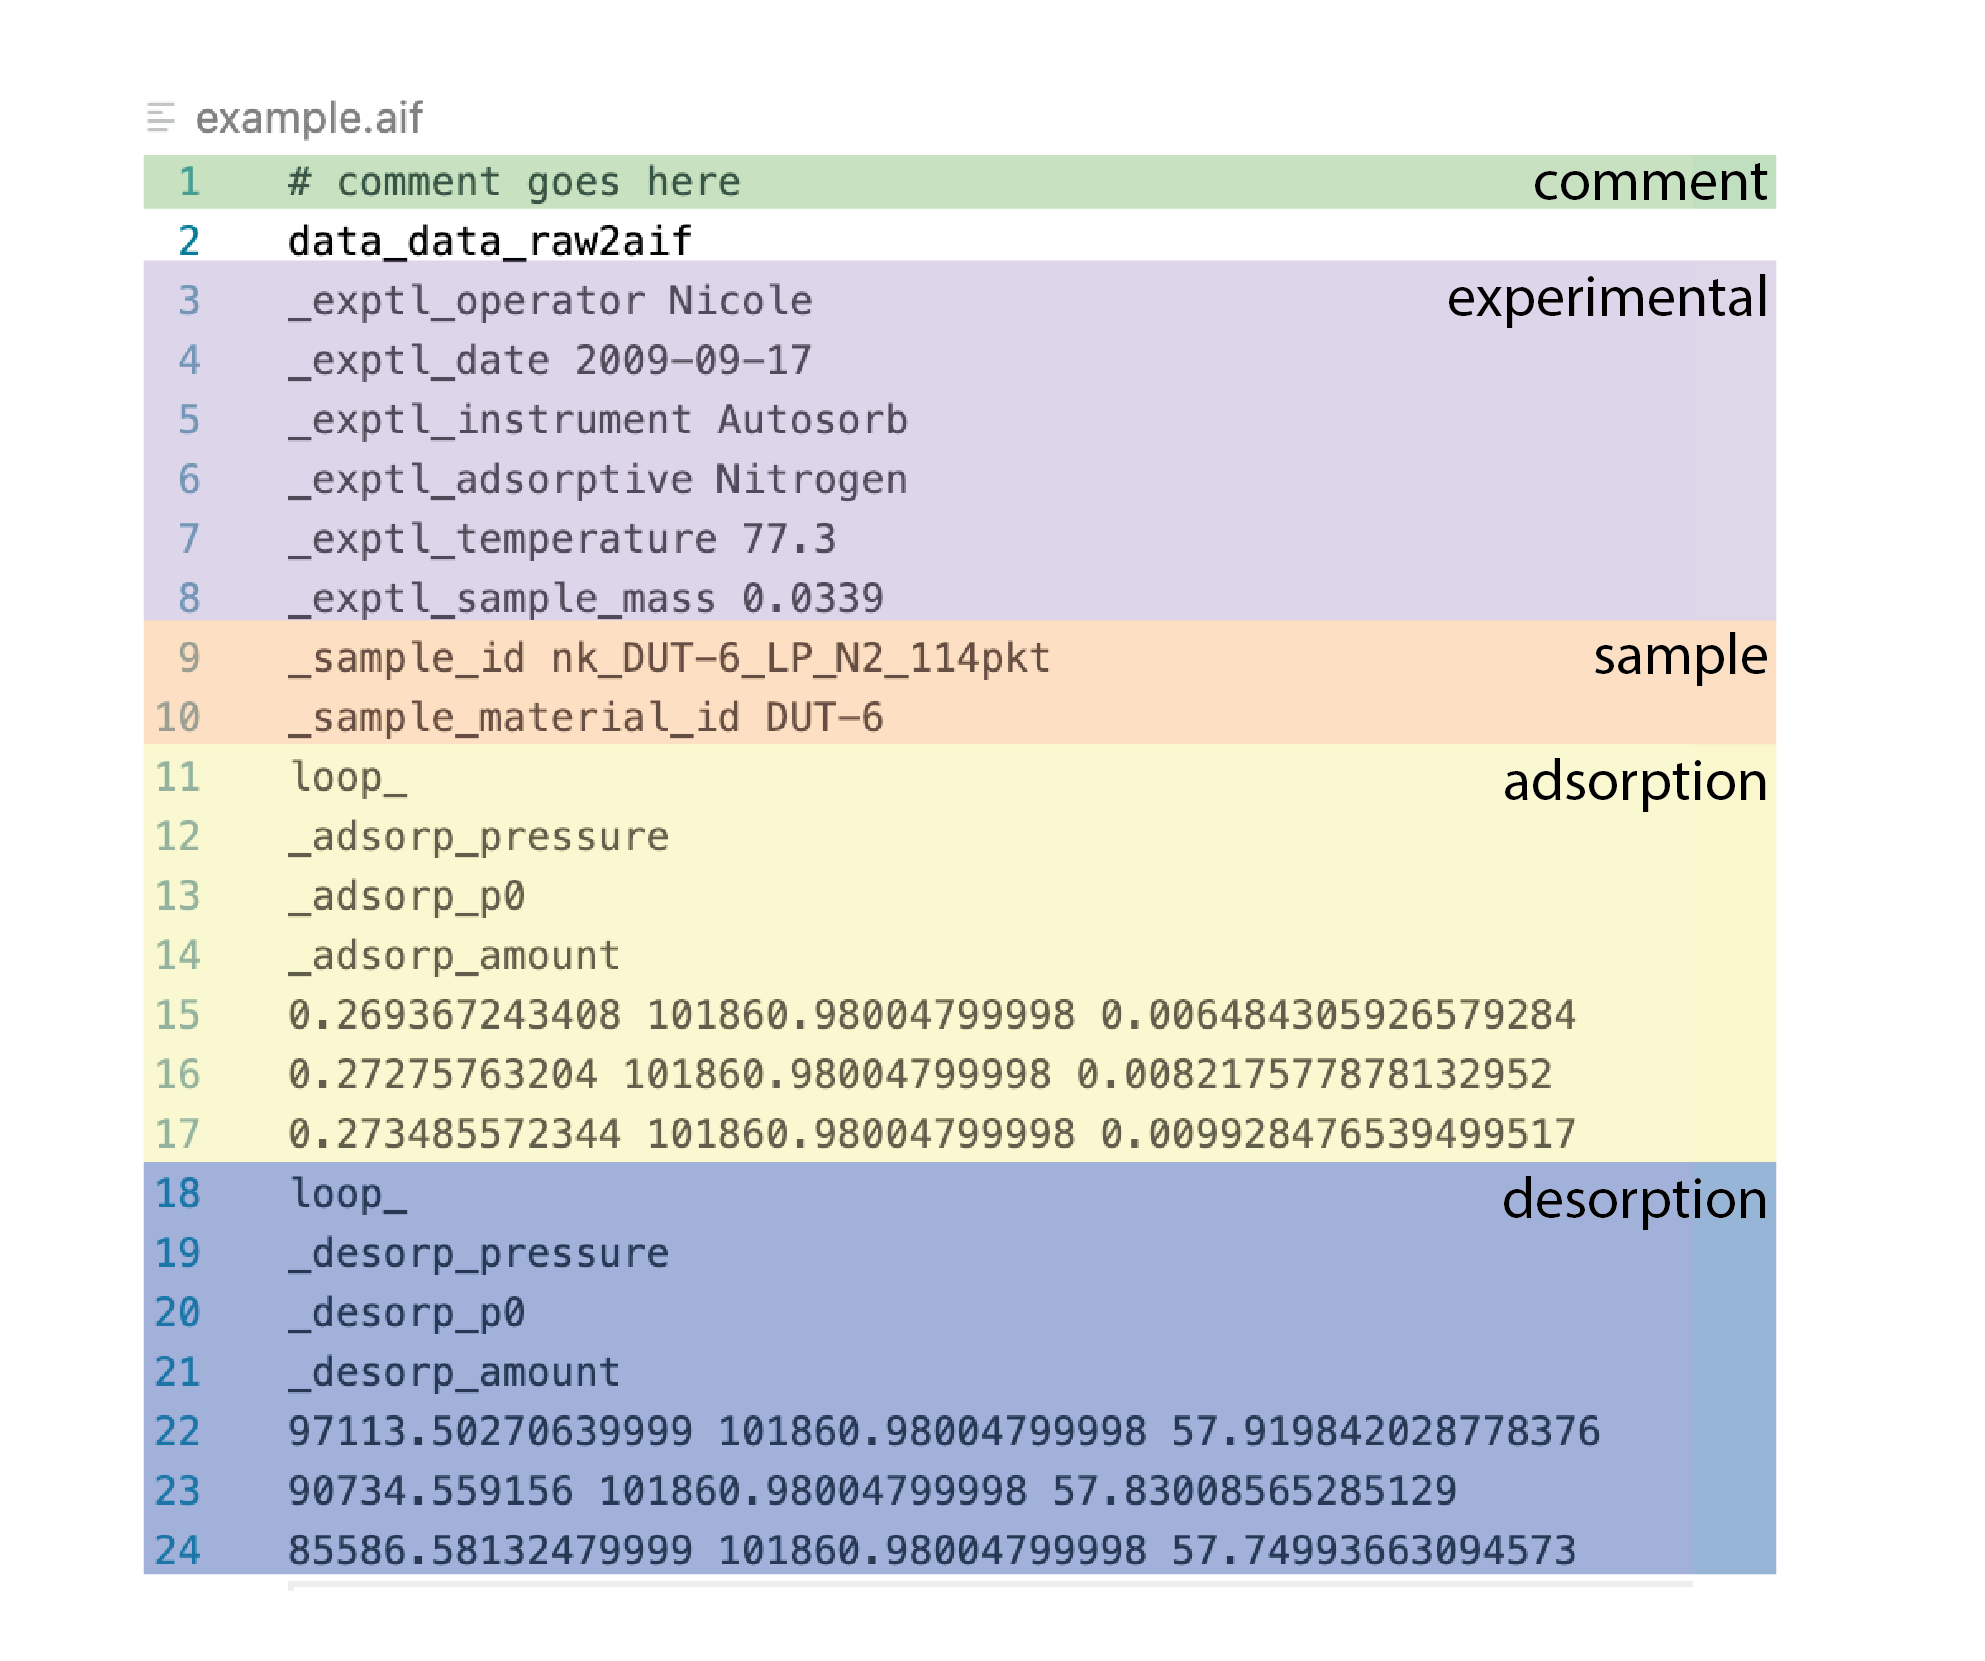
\includegraphics{./figures/structure-01.png}
      \caption{The structure of a typical adsorption information file (AIF) with the different data areas representing metadata (experimental and sample information) and the adsorption and desorption data.}
      \label{fgr:datastructure}
    \end{figure}


The above data structures of the STAR format prove ideal for describing the detailed quantities relating to an adsorption experiment.
An entire experiment can be described within a single data block.
Initially, data name and data value pairs can be used to identify quantities relating to the whole experiment such as the date and time, temperature and adsorptive.
The data points for the adsorption and desorption branch can then be detailed in separate data loops.
For each point, quantities such as the absolute pressure, relative pressure and amount adsorbed can be detailed.
This leads us to the general data structure for the AIF (Figure~\ref{fgr:datastructure}).


\section{AIF dictionary}
Each data item within a data block is identified using a unique data name.
The currently accepted AIF data names are listed and defined in Table~\ref{tbl:example}.
These data items form a first version of a core dictionary, which are intended for primarily reporting primary physisorption data.
As a result the dictionary contains information about crucial experimental parameters, basic sample characterization, adsorption and desorption measures, each distinguished by a data name prefix (\texttt{\_exptl\_}, \texttt{\_sample\_}, \texttt{\_adsorp\_} and \texttt{\_desorp\_}).

\begin{table}
  \renewcommand{\arraystretch}{1.5}
  \caption{Core dictionary of data items}
  \label{tbl:example}
  \begin{tabular}{lp{7cm}}
    \toprule
    data name & description  \\
    \midrule
    \texttt{\_exptl\_operator}  & name of the person who ran the experiment (string)  \\
    \texttt{\_exptl\_date} & date and time of the experiment (date-time string representation) \\
    \texttt{\_exptl\_instrument}  & instrument id used for the experiment (string)  \\
    \texttt{\_exptl\_adsorptive}  & name of the adsorptive (string)  \\
    \texttt{\_exptl\_temperature}  & temperature of the experiment (float)  \\
    \texttt{\_exptl\_sample\_mass}  & mass of the sample (float, gram) \\
    \texttt{\_sample\_id}  & unique identifying code used by the operator (string)\\
    \texttt{\_sample\_material\_name}  & designated name for the material (string) \\
    \texttt{\_adsorp\_pressure} & equilibrium pressure of the adsorption measurement (float, pascal)\\
    \texttt{\_adsorp\_p0} & saturation pressure of the adsorption measurement at the temperature of the experiment (float, pascal) \\
    \texttt{\_adsorp\_amount} & amount adsorbed during the adsorption measurement (float, mol$\,$kg$^{-1}$) \\
    \texttt{\_desorp\_pressure} & equilibrium  pressure of the desorption measurement (float, pascal) \\
    \texttt{\_desorp\_p0} & saturation pressure of the desorption measurement at the temperature of the experiment (float, pascal) \\
    \texttt{\_desorp\_amount} & amount adsorbed during the desorption measurement (float, mol$\,$kg$^{-1}$) \\
    \bottomrule
  \end{tabular}
\end{table}

The goal of the experimental data names is to capture the information required to accurately portray the results of experiment, which at the very minimum are the temperature and adsorptive.
As metadata should include information that may aid in identifying possible errors this also includes the mass of sample used in the experiment.
Additionally, data is included relative to the date, time and person responsible for the measurement to produce a general picture of the provenance of the experiment.

Details of the sample are recorded for comparison and to uniquely identify the sample that was used in the experiment.
Simply, this includes the sample identity code (\texttt{\_sample\_id}), a laboratory code used to record and represent the sample and a string relating to the general designation given to the material (\texttt{\_sample\_material\_name}).

For each data point measured during an adsorption experiment data can be stored that relates to the equilibrium pressure, the saturation pressure and the amount adsorbed. Importantly, these should be stored in units of pascal and mol$\,$kg$^{-1}$ to follow the IUPAC recommendations.\cite{10.1515/pac-2014-1117}
The saturation pressure can be recorded at each data point as we have discovered that some instruments will meausure and report this value for every point.

The above features serve as an example of the data that can be archived in a AIF and can be extended in future versions.
For example, the intention of this initial version is to provide digital archive of the presented primary data of an adsorption experiment, the isotherm.
As a result, it describes only basic information that usually exported from adsorption instruments and a few convenient metadata items.
The flexibility of this approach can be extended in future versions to include more detailed parameters not commonly presented, such as dead volume measurements and leak checks, or combined with CIF data names for structural data to archive parallelized adsorption-diffraction measurements.

\section{Creating and using the AIF}
A simple python 3.8 routine was prepared during the development of the AIF to convert the plain text data output from 3P instruments (formerly Quantachrome) and Microtrac Retsch (formerly BEL Japan and BEL Europe) instruments, used in many laboratories around the world.
Specifically, this has been written to parse raw analysis text files exported by Quantachrome software and the raw data files (\textit{.DAT}) and CSV files exported by Belsorb software.
Instrument manufacturers are encouraged to provide readable raw data files in future.
For example, it is currently not possible to read binary data files e.g. the files saved by 3P instruments (\textit{.qps}).
Our routine is easily transferable and will be adapted for other instruments in future.
The source code and a stand-alone program is provided on GitHub (\url{www.github.com/jackevansadl/adsorptioninformationfile}) and can be adapted individually by instrument manufacturers.
In future, we also plan to include as routine for the transformation of files produced by Micromeritics instruments.

This simple program will parse the output data to find data items detailed in the AIF dictionary.
These data items are converted to the appropriate units and the isotherm is split into the adsorption and desorption parts.
Subsequently an AIF is produced using \textit{gemmi} CIF routines.\cite{gemmi}
As a consequence routines and methods developed for treating CIF files can be used in this application to physisorption data.
For example, produced AIF files can also be read using existing CIF methods, such as the \texttt{gemmi} python library that is considered the fastest open-source CIF parser.\cite{gemmi}
We have used \texttt{gemmi} library to demonstrate how an isotherm can be displayed from an AIF using a few lines.
This is a very simple implementation and it is hoped that future versions, following the cooperation of several manufactures, could result in to routines to parse the information directly from binary data used by the instruments.

To illustrate the importance of a universal data format for adsorption data we can compare data contained within an AIF to data digitized from a figure in a manuscript, for the same experiment.
The porous material DUT-6 (also referred to as MOF-205) is a metal-organic framework produced from zinc nitrate and two different different ligands; 2,6-naphthalenedicarboxylate and benzene-1,3,5-tribenzoate.\cite{10.1002/anie.200904599}
DUT-6 has mesopores of 2.4~nm, with dodecahedral geometry, and smaller cages of 0.9~nm that produce an extremely porous material with large adsorption capacities for \textit{n}-butane (up to 1.1~g$\,$g$^{-1}$ at 293~K),  methane (230~mg$\,$g$^{-1}$ at 100~bar and 298~K) and hydrogen (60~mg$\,$g$^{-1}$ at 50~bar and 77~K).
The nitrogen adsorption isotherm at 77~K was reported in the original manuscript using relative pressure and a linear axis (Figure~\ref{fgr:example}a).
From this plot the isotherm can be classified  as  type  Ib, clearly exhibiting characteristics of a hierarchal pore system with micropores and mesopores.
There is evidently a distinct step $p/p_0$ = 0.17, however, from this plot it is not possible to correctly identify low pressure features.
The low pressure regions is important for understanding the process of sequential pore filling or for independent application of analysis methods, such as the Brunauer–Emmett–Teller (BET) method.\cite{10.1016/S0167-2991(07)80008-5}
The reported isotherm was digitized using WebPlotDigitizer, which uses a time-consuming but powerful point-picking methodology.\cite{webplotdigitizer}
In this methodology, each point in the graph is identified by clicking on the image area and the point's location in on-screen pixels is then converted to data values, based on an axes calibration.
The digitized isotherm and the data from the experiment, when plotted on semi-log axes, clearly shows important low pressure information, such as the point of initial pore-filling, is lost when this information is simply included as a figure in a manuscript (Figure~\ref{fgr:example}).

To prevent this information loss and to allow further analysis of reported adsorption experiments by other researchers, adsorption data should be archived and shared using a universal and complete data format like that of the AIF.

  
  \begin{figure}[htb]
    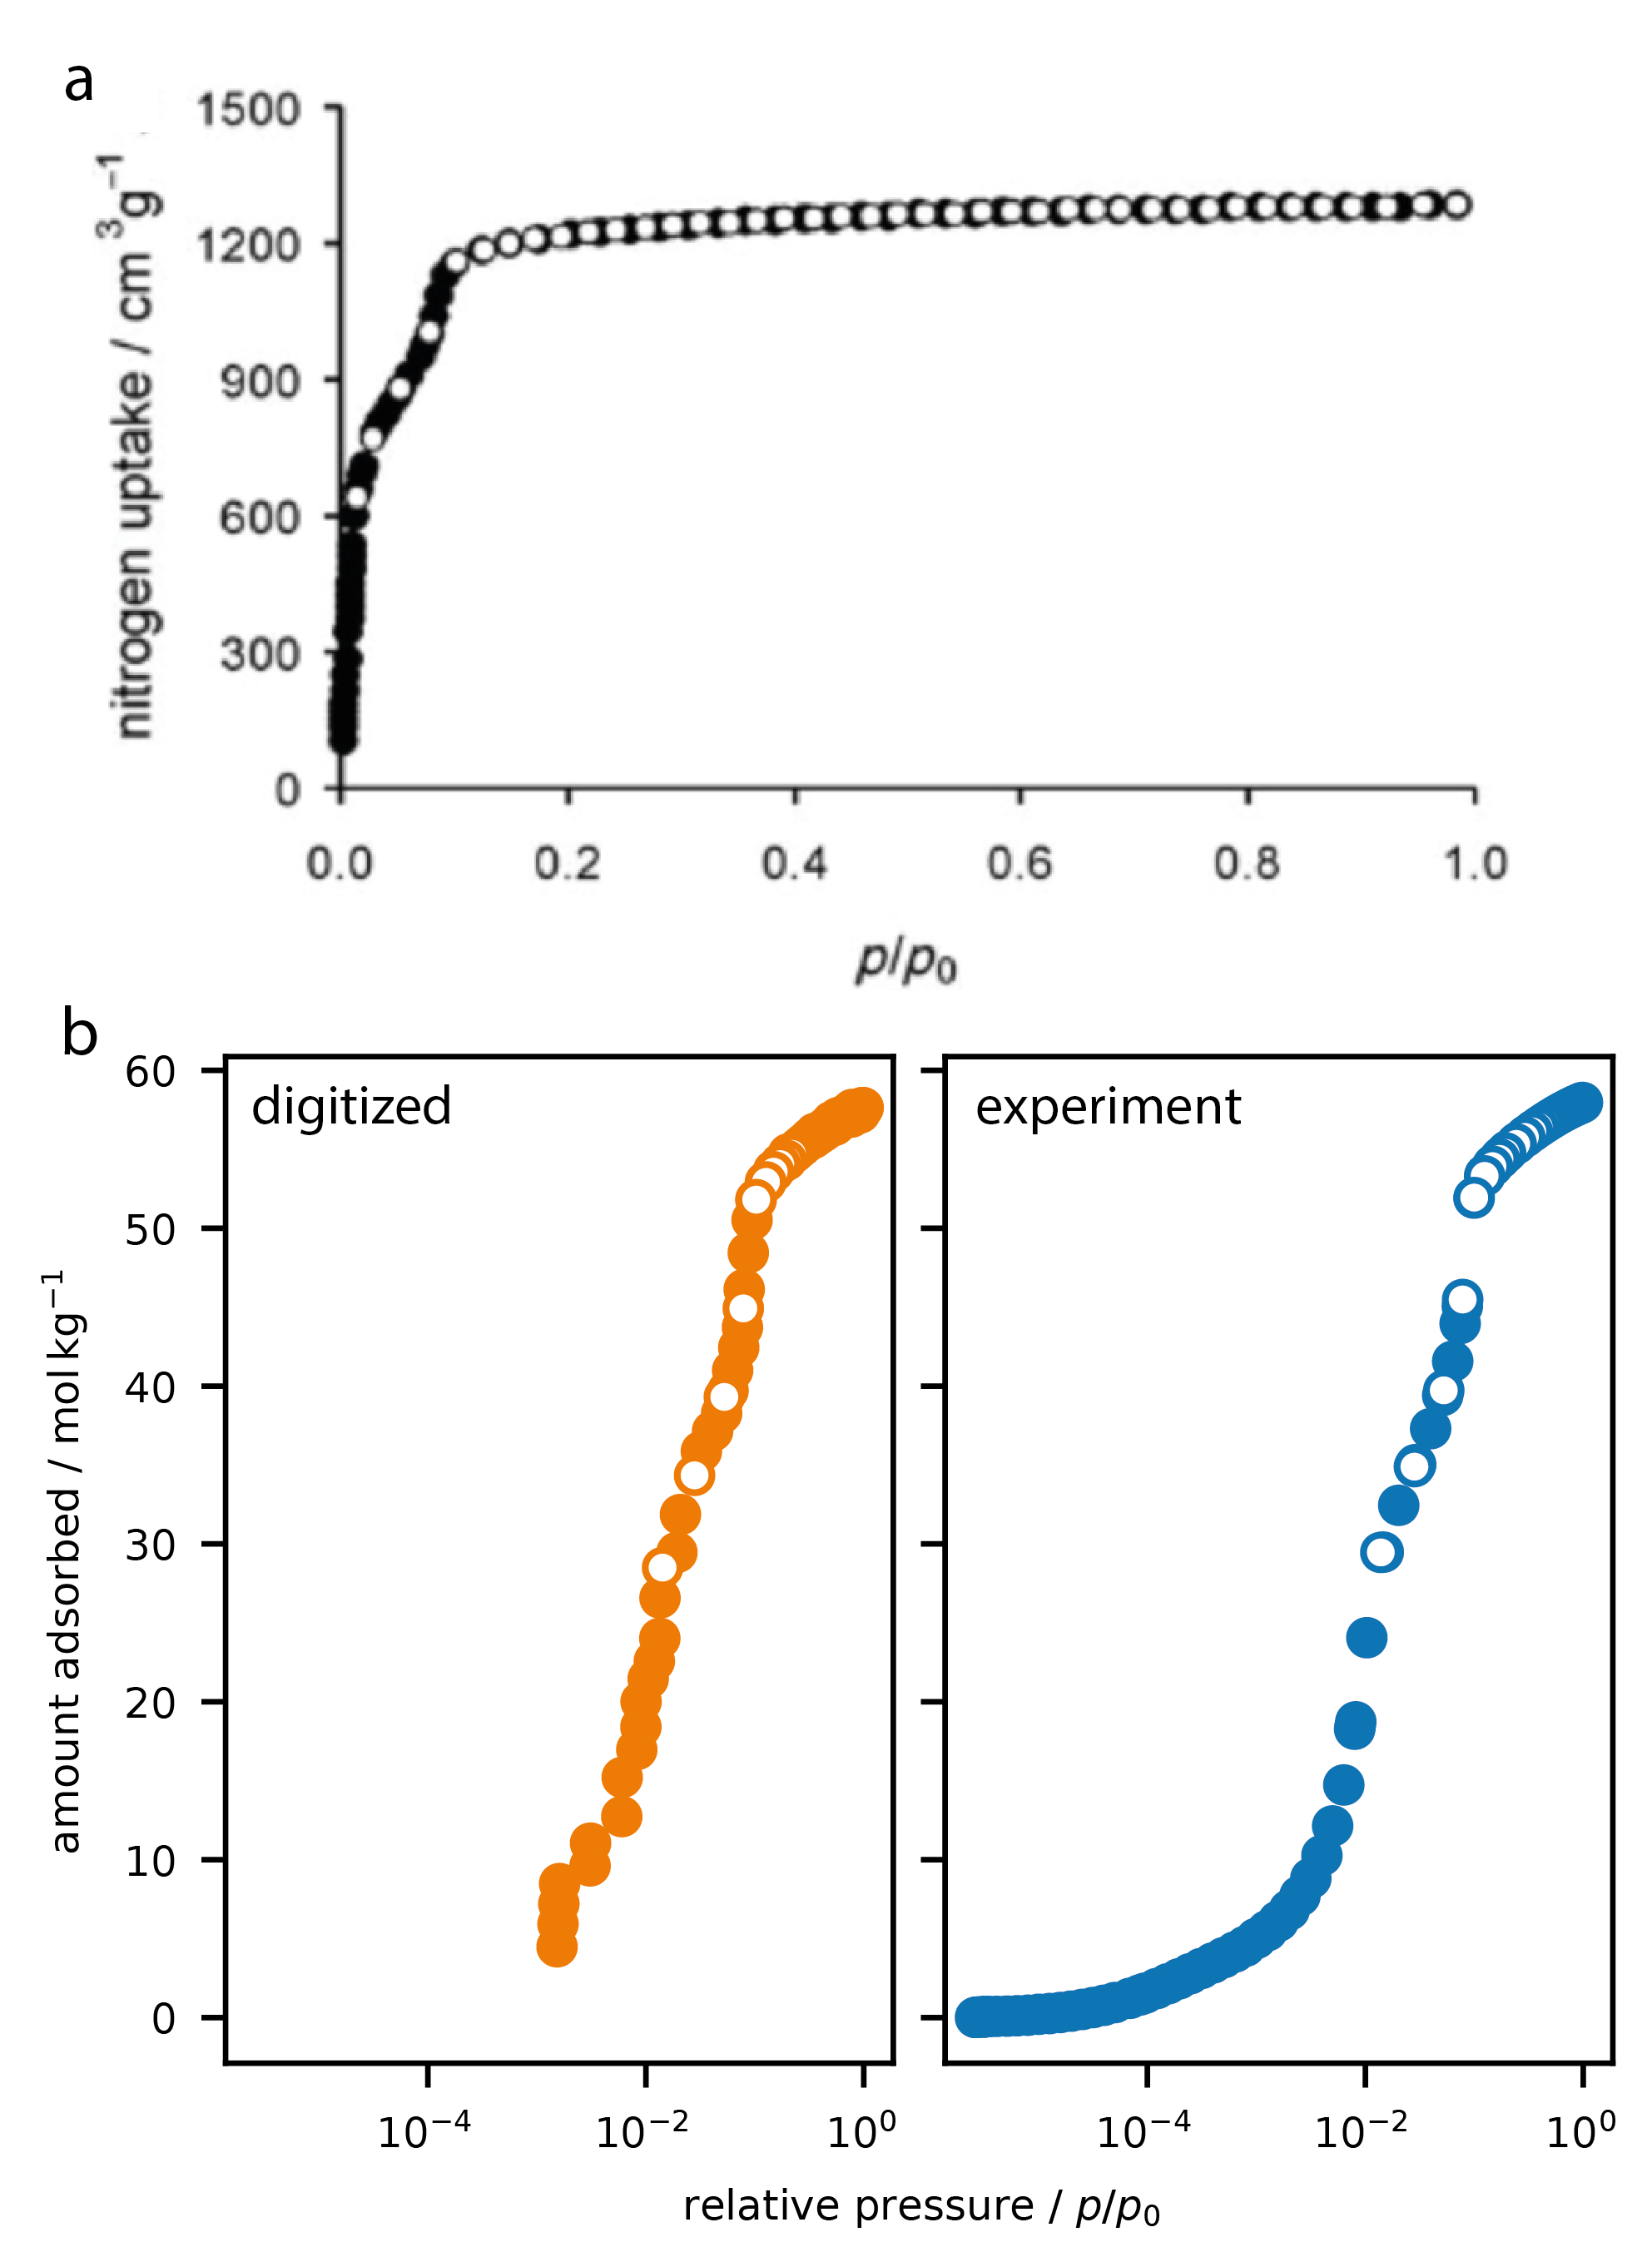
\includegraphics{./figures/example-01.png}
      \caption{The reported nitrogen adsorption isotherm of DUT-6 recorded at 77$\,$K (a) as reported in Ref. \citenum{10.1002/anie.200904599}. A digitized representation of this reported isotherm was achieved using a point-picking method (b) and compared to the experimental data as contained within an AIF (c).}
      \label{fgr:example}
    \end{figure}


\section{Summary and perspective}
There is a current need to develop a universal format for archiving adsorption data.
This is pertinent for the development of detailed databases of information that can play an important role in future materials design, application data mining, and for developing machine learning computational methods for adsorption processes. \cite{10.1021/acs.chemmater.9b03376}
This report details the specification of a new standard file, named AIF, based on the self-defining text archive and retrieval (STAR) procedure, inspired by similar universal and evolving formats currently used in the larger scientific community.
The AIF is importantly an easily extended free-format archive file that can be both human and machine readable.
This format represents the first steps to an open adsorption data format and the community is encouraged to take up this format.



%%%%%%%%%%%%%%%%%%%%%%%%%%%%%%%%%%%%%%%%%%%%%%%%%%%%%%%%%%%%%%%%%%%%%
%% The "Acknowledgement" section can be given in all manuscript
%% classes.  This should be given within the "acknowledgement"
%% environment, which will make the correct section or running title.
%%%%%%%%%%%%%%%%%%%%%%%%%%%%%%%%%%%%%%%%%%%%%%%%%%%%%%%%%%%%%%%%%%%%%
\begin{acknowledgement}
  J. D. E. acknowledges the support of the Alexander von Humboldt foundation and HPC platforms provided by a GENCI grant (A0070807069) and the Center for Information Services and High Performance Computing (ZIH) at TU Dresden.
  We thank Ren Koh for assistance with the development of the raw2aif file converter and Andrew Tarzia (University College London) for testing the program.
\end{acknowledgement}

%%%%%%%%%%%%%%%%%%%%%%%%%%%%%%%%%%%%%%%%%%%%%%%%%%%%%%%%%%%%%%%%%%%%%
%% The same is true for Supporting Information, which should use the
%% suppinfo environment.
%%%%%%%%%%%%%%%%%%%%%%%%%%%%%%%%%%%%%%%%%%%%%%%%%%%%%%%%%%%%%%%%%%%%%
% \begin{suppinfo}

% This will usually read something like: ``Experimental procedures and
% characterization data for all new compounds. The class will
% automatically add a sentence pointing to the information on-line:

% \end{suppinfo}

%%%%%%%%%%%%%%%%%%%%%%%%%%%%%%%%%%%%%%%%%%%%%%%%%%%%%%%%%%%%%%%%%%%%%
%% The appropriate \bibliography command should be placed here.
%% Notice that the class file automatically sets \bibliographystyle
%% and also names the section correctly.
%%%%%%%%%%%%%%%%%%%%%%%%%%%%%%%%%%%%%%%%%%%%%%%%%%%%%%%%%%%%%%%%%%%%%
\bibliography{article}

\end{document}